\subsection{\cplop{} Makeup}
\autoref{fig:species} shows the distribution of \cplop{} \isols{} considered in this study among its 53 different \spec{}.
\begin{figure}[t]
    \centering
    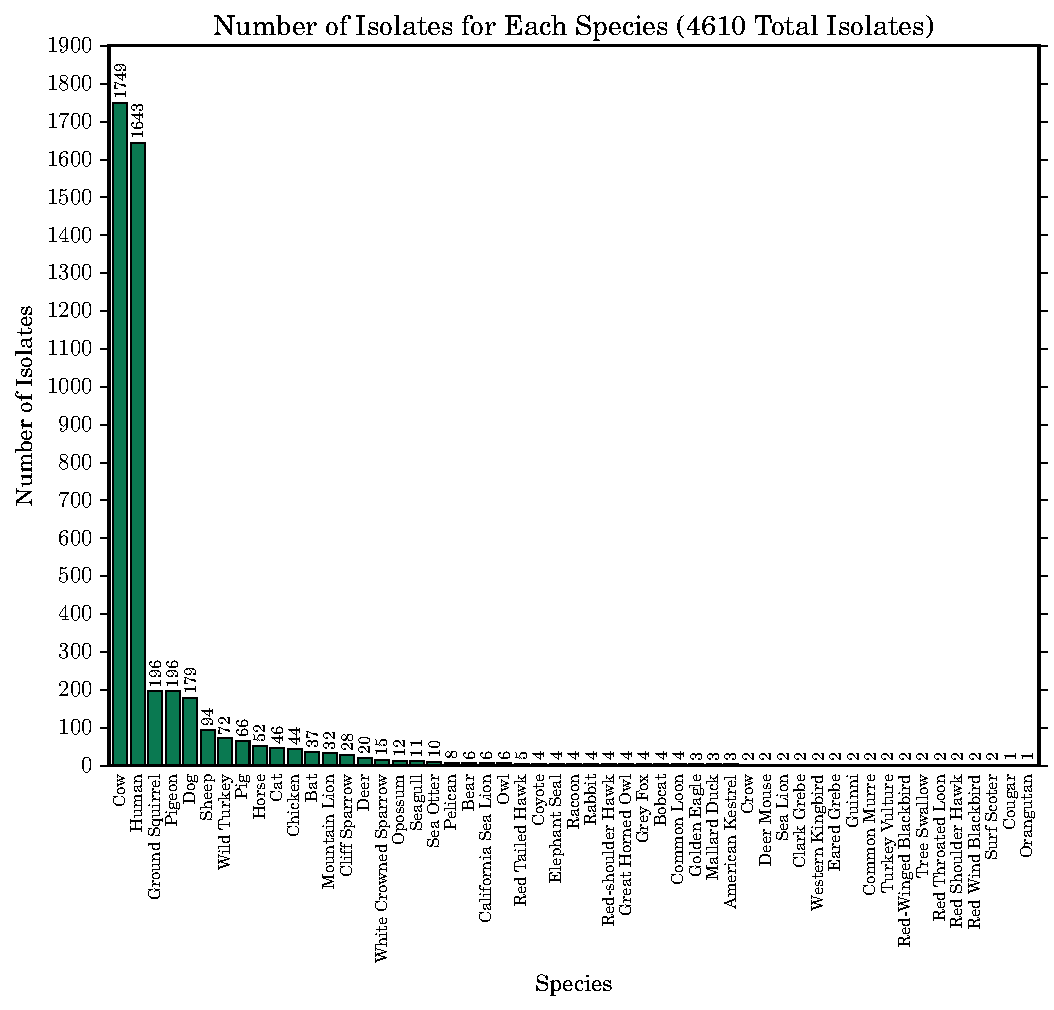
\includegraphics[width=\linewidth]{figures/bs/species_hist.pdf}
    \caption{
    A histogram of the number of \isols{} of each species in our study, taken from \cplop{}.
    There are 4,610 total \isols{} from 53 different \specs{}.}
    \label{fig:species}
\end{figure}

There are a total of 4,610 \isols{} in our dataset\footnote{A simplified version of \cplop{} containing \isol{} IDs, \spec{}, and \zscore{}s can be found at \texttt{https://github.com/jmcgover/cplop-acm-bcb-2016}.}. As seen from Figure \ref{fig:species},
the organic growth of \cplop{} yielded disproportionately many \ecoli{} isolates originating
from humans and cows (however, as shall be seen below, these isolates belong to a large number of strains). Each \isol{} is represented in \cplop{} with two \pyros{} ---  one each for \its{1} and \its{2} 
region.